\section{Evaluation in a Laboratory Setting}
\label{sec:evaluations_in_lab}

% We do not have to identify which exact part of the target device is responsible for the leakage, since we have already shown in Sec 4 that EVERYTHING LEAKS.

% The scope of this section is to show that the proposed attacks can be successfully conducted on several categories of real-world COST devices in a laboratory settings.
After analyzing xxx, we evaluate the performance of the proposed attack in this section.

\subsection{Experimental Setup}

\begin{figure}
    \centering
    \includegraphics[width=0.95\linewidth]{figures/5.1/setup1.pdf}
    \caption{Experiment setup \hr{change it to devices picture}}
    \label{fig:experiment setup}
\end{figure}

\Cref{fig:experiment setup} shows the experiment setup of the victim’s devices and adversary’s devices. The victim’s devices are analog-signal input/output devices widely deployed in daily life, making them representative targets in real-world settings. The adversary’s devices are used to inject fine-grained design signals to the victim devices to perform active side-channel analysis.

\textbf{Victim’s devices.} 
To evaluate the real-world performance of our attack on COSTs,
All devices are in their original enclosures without any hardware or software modifications to ensure the results reflect standard consumer deployments.
% We implement the attack on a variety of widely used analog-signal input/output devices, including 15 distinct COTS devices across 6 categories: wired headphones (Sony MDR-ZX110AP, JBL JBLT110, Apple Earbuds), wireless headphones (UGreen MAX2, PHILIPS TAH2020, HP H231R), microphones (UGreen CM769, Razer SEIREN V3 MINI), a wireless fixed phone (Flyingvoice), as well as smart home appliances including fans (OIDIRE ODI-MF10A, XIAOMI BPLDS10DM) and lamps (JD JINGZAO JDO-06, XIAOMI 1S). Specifically, the wired headphones were evaluated while connected to diverse host devices, including two laptops (Dell G5(5590H) and MacBook pro(M2)) and a smartphone (iPhone 15pro), to verify performance across different platforms. Notably, all evaluated COTS devices remain in their original enclosures, and no hardware or software modifications are made to the victim devices during our experiments.

\textbf{Adversary’s devices.} The adversary’s devices consist of two main components. The first is a signal injection module used to generate, amplify, and transmit carefully crafted injection signals to the victim devices. We choose a software defined radio(USRP B210) as transmitter and send a single tune carrier at varying frequencies ranging from 70~MHz to 2~GHz depending on the target device. The second is a receiving and analysis module used to receive the induced side-channel leakages and perform subsequent signal processing and side-channel analysis. We used a spectrum analyzer(siglent SSX 3075x Plus) to receive the reflected signal, observe and demodulate the sideband and export the baseband signal.

%分两类指标
% \textbf{Metrics.} We evaluate the attack performance using three key metrics: 
% (1) \textit{Injection Frequency}, which records the effective electromagnetic interference frequency for each device;
% (2) \textit{Signal-to-Noise Ratio (SNR)}, which quantifies the quality of the recovered signal at certain distance; and (3) \textit{Signal recognition rate}, defined as the proportion of successful injections out of total attempts. For audio devices, we played a single tune signal see if the signal can be recognized in the spetrum analyzer. For fan and lamp, we recognize the rotation speed and 50~Hz power frequency respectively. As shown in Table \ref{tab: Attacks on COTS Devices}, our method achieves a nearly 30/30 success rate across all tested devices.
\textbf{Metrics.} We define two categories of key metrics to evaluate the overall performance of the proposed injection-induced EM side-channel attack:
(1) \textit{Signal-to-Noise Ratio (SNR)} is d
(2) \textit{Signal recognition rate},
We report the vulnerable frequencies for each device under the test.

\subsection{Attacks on COTS devices}
% \qh{For each subsubsection, our writing strategy is as follows: (1) the first paragraph briefly introduce the sensitive real-world scenarios in which this type of device is commonly used; (2) in the second paragraph, we introduce the devices under our test and summarize the observed results and consequences; (3) in the third paragraph, we just discuss how these consequences could result in real-world incidents/harms. I provide an example in~\cref{sec:attacks_on_lamps} for reference.}

\begin{table*}[t]
\centering
\footnotesize
\renewcommand{\arraystretch}{1.3}

\begin{threeparttable}

\caption{Summary of Attacks on COTS Devices}
\label{tab: Attacks on COTS Devices}

\begin{tabular}{|l|l|l|c|c|c|c|c|c|}
\hline

% Header
\textbf{Device Type} & \textbf{Brand} & \textbf{Model} & \textbf{Year} & \textbf{\makecell[c]{Source\\of leaks}} & \textbf{\makecell[c]{Injection\\Frequency}} & \textbf{\makecell[c]{SNR \tnote{\ddag} }} & \textbf{\makecell[c]{Recog.\\Rate \tnote{\S}}} & \textbf{\makecell[c]{Max\\Dist. \tnote{\P}}} \\
\hline

% Wired Headphones
\multirow{3}{*}{\textbf{\makecell[l]{Wired\\Headphones}}}
& Sony + Dell\tnote{*} & ZX110AP & 2014 & \multirow{3}{*}{Amplifier} & 510--570\,MHz & 22.5\,dB & 30/30 & 5\,m \\ \cline{2-4} \cline{6-9}
& Sony + Mac\tnote{*} & ZX110AP & 2014 & & 220--260\,MHz & 14.5\,dB & 30/30 & 4\,m \\ \cline{2-4} \cline{6-9}
& Apple + iPhone\tnote{*}& Earbuds & 2016 & & 1160--1180\,MHz & 6.4\,dB & 29/30 & 1\,m \\
\hline

% Wireless Headphones
\multirow{3}{*}{\textbf{\makecell[l]{Wireless\\Headphones}}}
& UGreen\tnote{\dag} & MAX2 & 2024 & \multirow{3}{*}{Amplifier} & 900--980\,MHz & 23.8\,dB & 30/30 & 6\,m \\ \cline{2-4} \cline{6-9}
& PHILIPS & TAH2020 & 2025 & & 1590--1650\,MHz & 21.6\,dB & 30/30 & 6\,m \\ \cline{2-4} \cline{6-9}
& HP & H231R & 2023 & & 980--1020\,MHz & 20.7\,dB & 29/30 & 4\,m \\
\hline

% Landline
\textbf{\makecell[l]{Landline}} & Flyingvoice & P23GW & 2023 & \makecell[c]{ADC \&\\Amplifier} & 840--920\,MHz & 13.5\,dB & 30/30 & 3\,m \\
\hline

% Fan
\multirow{2}{*}{\textbf{Fan}}
& OIDIRE\tnote{\dag} & ODI-MF10A & 2023 & \multirow{2}{*}{\makecell{Switching\\MOSFET}} & 440--520\,MHz & 39.1\,dB & 30/30 & 6\,m \\ \cline{2-4} \cline{6-9}
& XIAOMI & BPLDS10DM & 2025 & & 530--610\,MHz & 30.5\,dB & 30/30 & 4\,m \\
\hline

% Lamp
\multirow{2}{*}{\textbf{Lamp}}
& JINGZAO & JDO-06 & 2024 & \multirow{2}{*}{\makecell{Power\\Converter}} & 80--650\,MHz & 20.7\,dB & 29/30 & 3\,m \\ \cline{2-4} \cline{6-9}
& XIAOMI\tnote{\dag} & 1S & 2019 & & 70--700\,MHz & 22.4\,dB & 30/30 & 3\,m \\
\hline

\end{tabular}

% 关键修改:添加了 [para] 选项
\begin{tablenotes}[para]
    \footnotesize
    \item [*] Three different host devices for wired headphones.
    \item [\dag] Devices evaluated in \cref{sec: Impact Quantifications}.
    \item [\ddag] SNR is evaluated at 20\,cm distance.
    \item [\S] Recognition rate is evaluated at 20\,cm distance.
    \item [\P] Max distance is evaluated at 5/30 recognition rate.
\end{tablenotes}

\end{threeparttable}
\end{table*}




% \begin{figure}[t] % 使用 [t] 让图片顶端对齐,通常单栏图片放顶部最美观
%     \centering
    
    % % --- 第一行 ---
    % % 左上图
    % \begin{subfigure}[b]{0.48\linewidth} % 宽度设为当前栏宽的48%
    %     \centering
    %     \includegraphics[width=\linewidth]{figures/5.2/RES_Original.pdf} % 图片填满子图框
    %     \caption{Original Spectrum \hr{limit it to 4KHz}}
    %     \label{fig:original headphone }
    % \end{subfigure}
    % \hfill % 撑开两图之间的空隙
    % % 右上图
    % \begin{subfigure}[b]{0.48\linewidth}
    %     \centering
    %     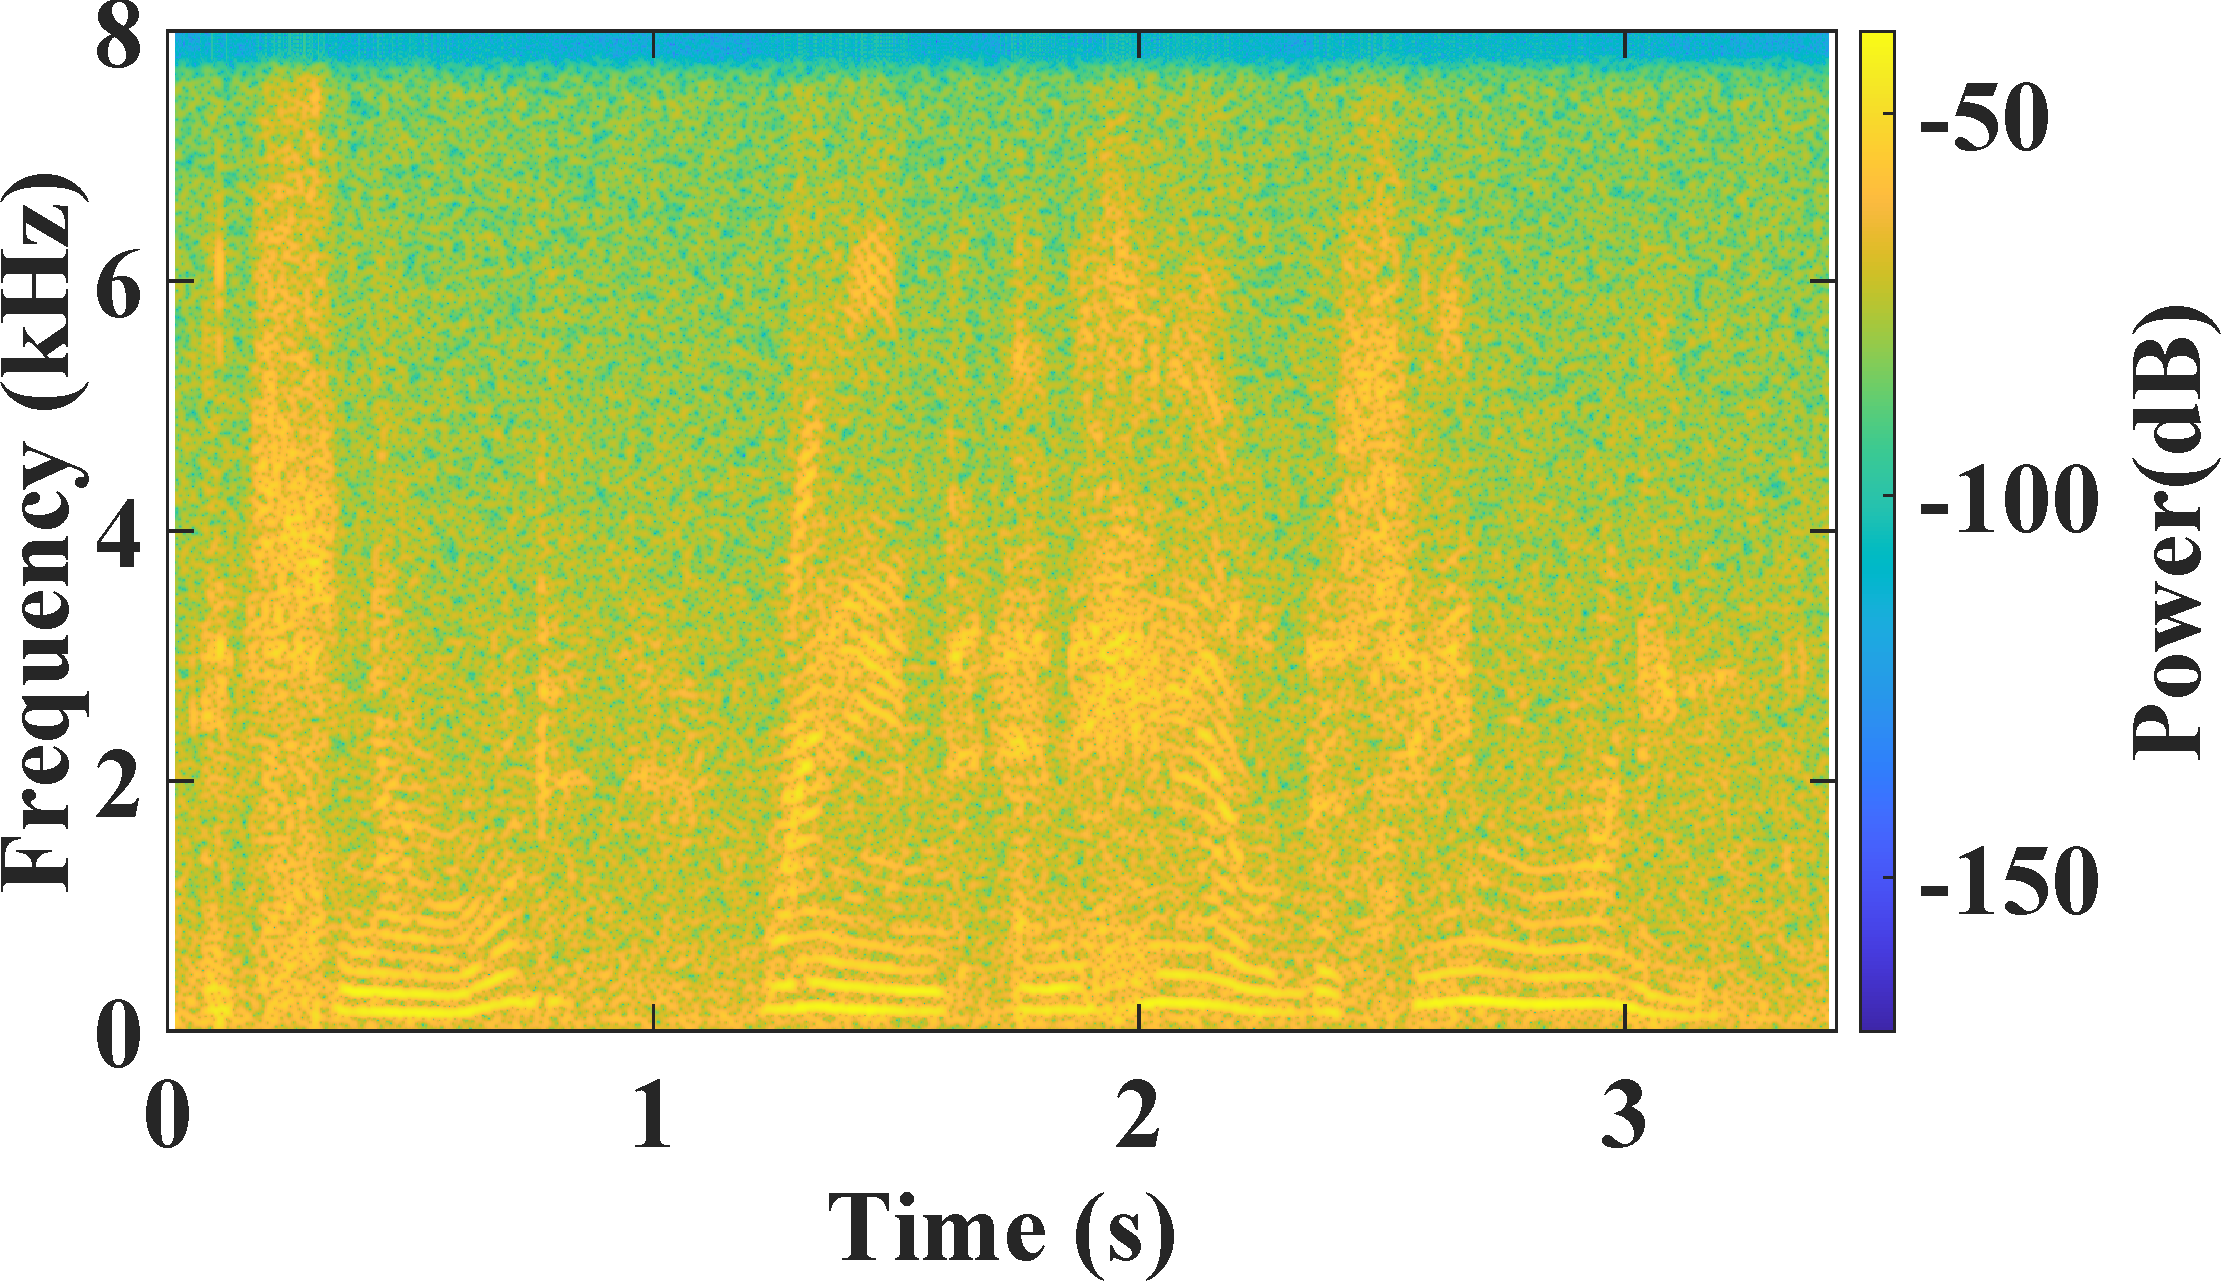
\includegraphics[width=\linewidth]{figures/5.2/RES_Headphone.pdf}
    %     \caption{Recieved Spectrum}
    %     \label{fig:recieved headphone}
    % \end{subfigure}

    % \vspace{3mm} % 调整上下两行的间距
    
    % % --- 第二行 ---
    % % 左下图
    % \begin{subfigure}[b]{0.48\linewidth}
    %     \centering
    %     \includegraphics[width=\linewidth]{figures/placeholder.pdf}
    %     \caption{Original Spectrum}
    %     \label{fig:original microphone}
    % \end{subfigure}
    % \hfill
    % % 右下图
    % \begin{subfigure}[b]{0.48\linewidth}
    %     \centering
    %     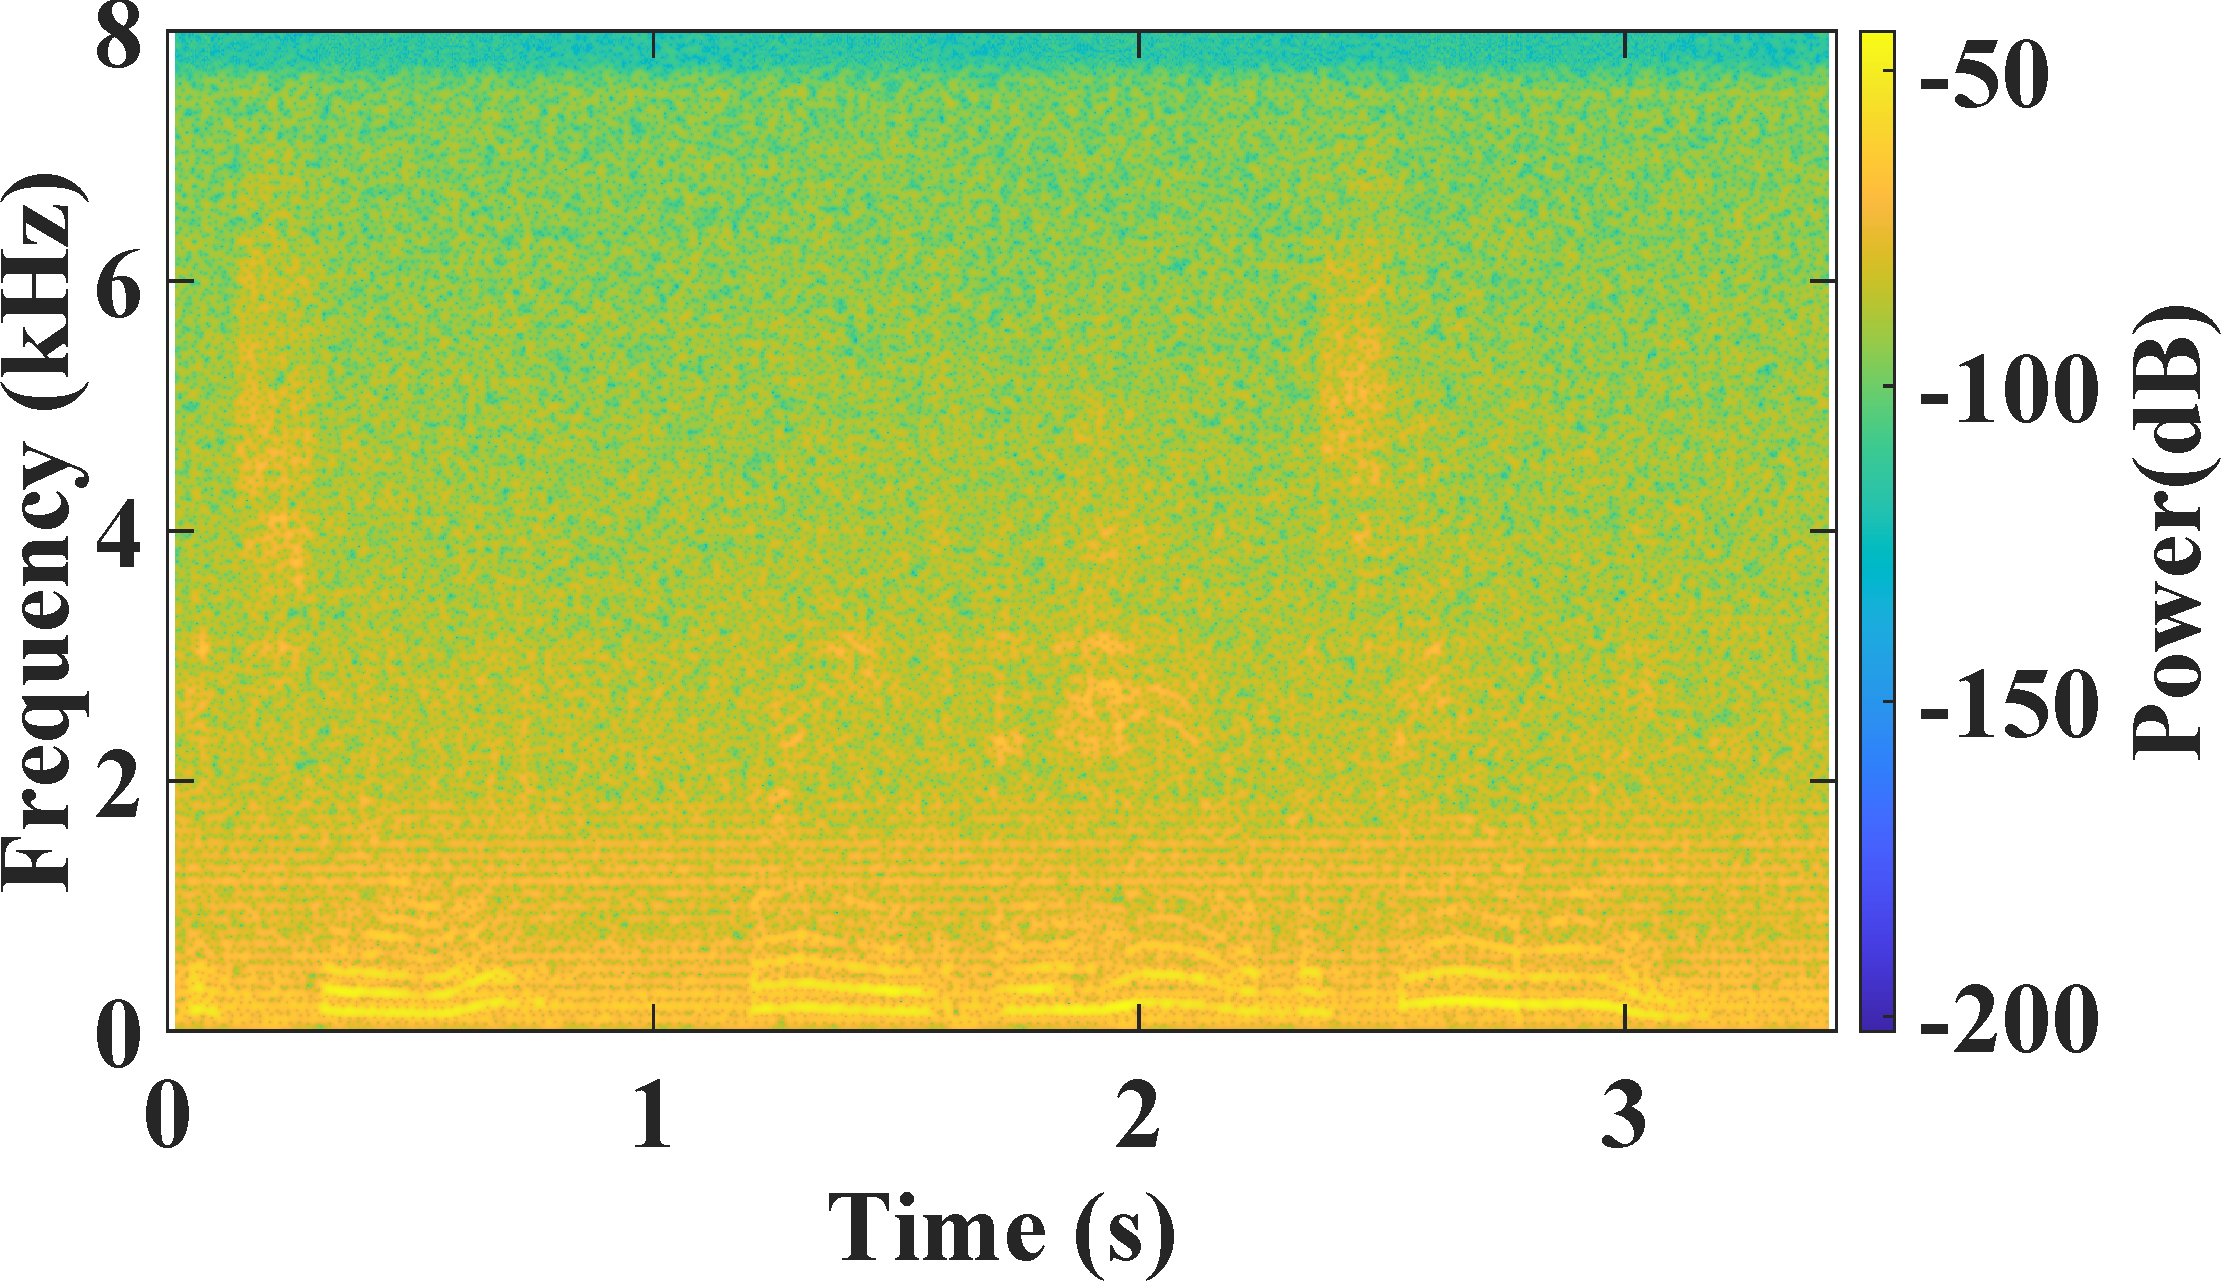
\includegraphics[width=\linewidth]{figures/5.2/RES_Microphone.pdf}
    %     \caption{Recieved Spectrum}
    %     \label{fig:recieved microphone}
    % \end{subfigure}

%     % --- 行间距 ---
%     \vspace{3mm} % 调整上下两行的间距
    
%     % --- 第二行 ---
%     % 左下图
%     \begin{subfigure}[b]{0.49\linewidth}
%         \centering
%         \includegraphics[width=\linewidth]{figures/5.2/RES_LAMP.pdf}
%         \caption{Lamp}
%         \label{fig:lamp}
%     \end{subfigure}
%     \hfill
    
%     % 右下图
%     \begin{subfigure}[b]{0.49\linewidth}
%         \centering
%         \includegraphics[width=\linewidth]{figures/5.2/RES_FAN.pdf}
%         \caption{Fan \ly{Uncleare what this figure means. What is the MHz frequency?}}
%         \label{fig:fan}
%     \end{subfigure}
    
%     \caption{Attacks on COTS devices.}
%     \label{fig:Attacks on COTS devices.}
    
% \end{figure}


\subsubsection{Attacks on Headphones}
% Headphones, encompassing both wired and wireless variants, are ubiquitous in personal and professional environments, serving as the primary interface for confidential voice communication. They are extensively used for VoIP calls, virtual conferences, and private media consumption in offices, government facilities, and public spaces. Users typically rely on headphones to prevent audio leakage to the immediate environment, operating under the assumption that the audio stream is secure—protected either by physical isolation in wired headsets or digital encryption protocols in Bluetooth headsets. Consequently, these devices often handle highly sensitive information, making them high-value targets for eavesdropping.

% To evaluate the vulnerability of these devices, we conducted experiments on a diverse set of representative models, including wired headsets (Sony MDR-ZX110AP, JBL T110) connected to two laptops (Dell G5(5590H), MacBook pro(M2)) respectively, and wireless models (UGreen MAX2, PHILIPS TAH2020, Lenovo EH410). As summarized in \cref{tab: Attacks on COTS Devices}, our results demonstrate that both categories are susceptible to the proposed attack. Take PHILIPS TAH2020 as an example, we achieved a Signal-to-Noise Ratio (SNR) of up to 37.8dB by injecting a 170MHz signal. In all cases, we were able to recover intelligible audio.\cref{fig:Attacks on COTS devices.} visually confirms these findings, where the recovered spectrum (\cref{fig:recieved headphone}) exhibits a strong correlation with the original audio spectrum (\cref{fig:original headphone}).

% The ability to recover high-fidelity audio from these devices poses a severe security threat. This attack effectively circumvents standard protections: for wired devices, it breaches the perceived air-gap security; for wireless devices, it bypasses Bluetooth encryption by targeting the post-decryption analog stage. This implies that an adversary can eavesdrop on sensitive conversations—such as business negotiations or private calls—without physical access to the victim's device, without installing malware, and regardless of the underlying operating system or software encryption. The compromised headphones essentially function as remote broadcasting devices, leaking private audio to any attacker within the effective range. \hr{I need to find close-loop control examples}
\begin{figure}[t]
    \centering
    \includegraphics[width= 1.0\linewidth]{figures/5.2/RES.pdf}
    \caption{Attack on headphone.}
    \label{fig:recieved headphone}
\end{figure}
Headphones represent the ``last mile'' of audio security. Whether wired or wireless, they are trusted to keep audio streams private, often handling sensitive content from VoIP calls and classified meetings. The prevailing security assumption is that wired connections are air-gapped from network attackers, while wireless connections are protected by strong cryptographic protocols (e.g., Bluetooth encryption). We challenge this assumption by targeting the analog circuitry that exists after decryption and before sound generation.

We evaluated our injection attack on a diverse set of headphones, including wired models connected to various hosts and wireless models. As shown in \cref{tab: Attacks on COTS Devices}, we achieved a 100\% signal recognition rate across almost all 9 test configurations.
The attack exploits the non-linearity of the headphone's internal amplifier. By injecting a single tune carrier signal to the headphone cabling, we induce intermodulation that up-converts the analog audio signal. 
For instance, targeting the wireless PHILIPS TAH2020 with a $1620\text{ MHz}$ carrier yielded a remarkably high SNR of $21.6\text{ dB}$. 
% Similarly, the wired Sony MDR-ZX110AP yielded an SNR of $33.5\text{ dB}$ at $540\text{ MHz}$. 
In all cases, the recovered side-channel leakage contained intelligible speech with high spectral fidelity, as visualized in \cref{fig:recieved headphone}.

The ability to recover high-fidelity audio from these devices exposes a critical ``Post-Decryption'' vulnerability. For wireless headphones, our attack extracts the audio signal from the analog stage after the Bluetooth stack has decrypted it. This renders the communication protocol's encryption irrelevant to the physical-layer adversary. For wired headphones, the attack bridges the physical air-gap, allowing a remote adversary to eavesdrop without physical access or malware installation. Effectively, the hardware non-linearity transforms the victim's private listening device into a high-quality, long-range broadcasting station.

% \subsubsection{Attacks on Microphones}
% % External microphones serve as the gold standard for high-quality audio acquisition, widely deployed in live streaming, gaming, and critical teleconferencing. Due to their performance advantages over built-in alternatives, they are frequently installed in high-security settings, including executive offices and meeting rooms. Serving as the initial entry point for voice data, these devices capture sensitive audio at the source—from confidential strategies to intimate conversations. Crucially, this usage is predicated on a fragile trust model: users typically assume that unless a device is compromised by malware or physically tapped, their audio feed remains secure, overlooking physical-layer vulnerabilities.

% % To investigate the privacy risks associated with these input devices, we evaluated two popular commercial microphones: the UGreen CM769 and the Razer SEIREN V3 MINI. Our experiments focused on recovering the analog voice signals generated by the microphone capsule before they are digitized and encrypted by the host system. As indicated in \cref{tab:cots_attacks}, our method successfully reconstructed clear audio signals from both tested models. The attack exploits the electromagnetic coupling in the microphone's internal pre-amplification circuitry and cabling. The effectiveness of this extraction is visualized in \cref{fig:Attacks on COTS devices.}, where the received spectrum shown in \cref{fig:bot_right} demonstrates a clear recovery of the voice signature compared to the original input.


% % The vulnerability of microphones to this side-channel attack represents a critical breach of user privacy, as it allows for "input eavesdropping." Unlike headphone attacks which recover what the user hears, this attack recovers what the user says. Consequently, an adversary can remotely turn a victim's high-quality microphone into a covert listening device. This is particularly dangerous because the leakage occurs at the physical layer, meaning the attack is effective even if the host computer is secure, malware-free, or if the communication software employs end-to-end encryption. The ability to passively capture voice data from a distance fundamentally undermines the confidentiality of secure physical spaces where these devices are deployed.\hr{I need to find close-loop control examples}
% Microphones represent the input interface for sensitive user data, capturing everything from confidential voice commands to private negotiations. While software-level protections (e.g., OS permission flags, end-to-end encryption) secure the digitized data stream, the analog signal path prior to digitization remains vulnerable. We target this pre-digital analog stage, treating the microphone's internal pre-amplification circuitry as an unintentional modulator.

% We tested two popular external microphones (UGreen CM769, Razer SEIREN V3 MINI) commonly found in home-office setups. Our injection attack successfully reconstructed clear, intelligible audio from both devices, with the Razer model yielding an SNR of $15.2\text{ dB}$ at a distance of $0.5\text{m}$. The mechanism relies on the strong coupling between the injected carrier (e.g., $710\text{ MHz}$) and the microphone's analog cabling and pre-amplifier. The non-linearity of the pre-amp modulates the acoustic signal onto the carrier before it reaches the ADC. As shown in \cref{fig:original microphone} \cref{fig:recieved microphone}, the spectral features of the recovered voice signature are highly correlated with the original input, allowing for high-accuracy speech recovery.

% Attacks on microphones introduce a distinct ``Input Eavesdropping'' threat model that differs fundamentally from headphone leakage: Unlike headphones (which leak what the user hears), this attack captures what the user says. This enables the theft of authentication factors (voice biometrics), voice commands, and one-sided conversation data. Because the leakage occurs in the physical layer (analog circuit) before the ADC, the attack remains effective even if the host computer is fully secured, malware-free, or if the microphone is ``muted'' in software but powered electrically.

\subsubsection{Attacks on Fan}
Smart fans have evolved from simple cooling appliances into context-aware IoT devices, often featuring distinct modes like ``Sleep Mode'' (low noise/speed), ``Natural Breeze'' (variable speed), or ``Standard'' (constant speed). Much like smart lamps, the operational state of a fan serves as a direct proxy for the user's immediate environment and behavioral context. We investigated whether the electromagnetic leakage from the fan's motor control could expose these sensitive states.

We evaluated the OIDIRE ODI-MF10A and XIAOMI BPLDS10DM smart fans. As shown in \cref{tab: Attacks on COTS Devices}, the OIDIRE model proved highly susceptible, yielding an SNR of $37.9\text{ dB}$ at a distance of $8\text{ m}$.The attack exploits the modulation effect caused by the motor's driving signal. The fan's rotational speed(low:31Hz medium:42Hz high:52Hz) acts as a low-frequency characteristic that modulates the injected carrier (e.g., $480\text{ MHz}$). \ly{what is the baseband secret's frequency?}\hr{Added} Unlike the amplitude-based leakage in lamps, the fan's leakage manifests in the frequency domain. As visualized in~\cref{fig:Attacks on COTS devices.}, different speed settings generate sidebands at distinct frequency offsets. 

The ability to remotely discern specific fan speeds enables ``Context Inference'' attacks similar to those on smart lighting: Specific fan modes map to user activities. For instance, detecting a consistent ``Low'' speed (Sleep Mode) at night confirms the user is resting, while a ``High'' speed might indicate active daytime usage or a crowded room requiring maximum cooling. An adversary can log usage patterns over time (e.g., when the fan switches from ``Standard'' to ``Natural Breeze'') to build a detailed routine of the victim's daily life, inferring occupancy and sleep schedules without visual surveillance.

\begin{figure}[t]
    \centering
    \includegraphics[width= 1.0\linewidth]{figures/5.2/attacks_lamp_fan.pdf}
    \caption{Attacks on COTS devices.}
    \label{fig:Attacks on COTS devices.}
\end{figure}

% \qh{Suvery some examples to claim we can enable Closed-loop Control of EM Injection and Eavesdropping if we know the speed of the fan.}

\subsubsection{Attacks on Lamps}
\label{sec:attacks_on_lamps}

Smart lamps serve as integral components of the IoT ecosystem, where specific lighting ``scenes'' (e.g., ``Focus Mode'' vs. ``Reading Mode'') map directly to user activity. While seemingly benign, the power state of a smart lamp acts as a high-fidelity proxy for user presence and behavioral context. We investigated whether the power consumption signature of these devices could be recovered via EM injection to leak fine-grained state information.

We evaluated the Xiaomi 1S and JD JINGZAO JDO-06 smart lamps. As indicated in \cref{tab: Attacks on COTS Devices}, the Xiaomi 1S exhibited the strongest leakage among all tested devices, achieving an SNR of $49.1\text{ dB}$ at a distance of $5\text{ cm}$. The mechanism exploits the non-linearity of the lamp's power adapter (specifically the rectifier diodes). The AC mains current ($50\text{ Hz}$) acts as a baseband "secret" that modulates the injected carrier (e.g., $100\text{ MHz}$). Because the amplitude of the $50\text{ Hz}$ current draw is proportional to the lamp's power load, the resulting intermodulation sidebands (at $f_{carrier} \pm 50\text{ Hz}$) encode the precise dimming level. Our measurements confirmed a strong linear relationship ($R^2 \approx 0.98$) between the lamp's brightness percentage and the amplitude of these sidebands. As visualized in \cref{fig:lamp}, the sideband peaks grow proportionally with the luminous output, allowing us to remotely measure the exact brightness level.

The ability to infer precise power consumption transforms a light source into a ``Behavioral Profiling'' beacon: By mapping the recovered power levels to vendor-specific presets (e.g., 20\% brightness = ``Relaxation'', 100\% brightness = ``Work''), an adversary can infer the user's specific activity and schedule without visual access. This fine-grained data on power can also facilitate multi-modal attacks. For instance, knowing the exact lighting frequency and intensity can help calibrate optical side-channel attacks that extract cryptographic keys from power LEDs, as demonstrated in prior work.



\subsection{Impact Quantifications}

% \hr{I will adjust the detailed data.}
% To quantify attack performance under the impact of injection distance, injection power, antenna position, and the presence of barriers between the victim device and adversary.
% \qh{Here, we only need to conduct the evaluations on four representative devices, namely one headphone, one microphone, one fan, and one lamp.}

% \ly{Based on the hypothesized attack scenarios for each category of device analyzed above, ...} To establish a unified evaluation standard across diverse target types, including audio devices (e.g., headphones, microphones) and state-based appliances (e.g., lamps, fans), we define the Attack Success Rate (ASR) as the fidelity of the recovered information relative to the ground truth:
% \begin{equation}
%     \text{ASR} = 
%     \begin{cases} 
%         1 - \text{WER}, & \text{for Audio (e.g., Headphones),} \\ 
%         {N_{\text{correct}}} / {N_{\text{total}}}, & \text{for State (e.g., Lamps, Fans),} 
%     \end{cases}
% \end{equation}
% where $\text{WER}$ denotes the Word Error Rate in speech-to-text recovery, and $N_{\text{correct}}$ represents the number of correctly classified instances out of $N_{\text{total}}$ samples for discrete states. 
% %(e.g., distinguishing fan speeds via frequency shifts, or brightness levels via amplitude variations).
% For example, we can infer a fan’s rotational speed from the sideband frequencies, and estimate a desk lamp’s brightness from the peak amplitudes of the sidebands. Furthermore, using the above information, we can classify the operating states of such smart home devices.

% Unless otherwise specified, our default experimental configuration was set as follows to ensure consistency across all trials. The adversary's transmission and receiving antennas were positioned at a \textbf{distance} of 50~cm(for headphone and fan) and 10~cm(for microphone and lamp) \ly{move lamp to the 50~cm category, and need to re-organize reconsider microphone} from the target. The \textbf{angle of two antennas} was fixed at 45$^\circ$. The \textbf{injection power} (transmission gain) was set to a baseline of \underline{\hspace{0.8cm}} dB. For audio targets (Headphones), the output volume was standardized to a consistent sound pressure level (SPL) of 90~dB. \ly{90 dB is an unusually high volume, which will definitely cause questions} 
Based on the hypothesized attack scenarios for each category of device analyzed above, we proceed to quantify the real-world impact of injection-induced side channels. To establish a unified evaluation standard across diverse target types—ranging from analog audio devices such as headphones to state-based appliances such as lamps and fans—we define the \textbf{Attack Success Rate (ASR)} as the fidelity of the recovered information relative to the ground truth:

\begin{equation}
    \text{ASR} = 
    \begin{cases} 
        1 - \text{WER}, & \text{for Headphones,} \\ 
        N_{\text{correct}} / N_{\text{total}}, & \text{for Lamps and Fans,} 
    \end{cases}
\end{equation}

where $\text{WER}$ denotes the Word Error Rate in speech-to-text recovery, and $N_{\text{correct}}$ represents the number of correctly classified instances out of $N_{\text{total}}$ samples for discrete states. For example, we infer a fan’s rotational speed from the frequency shift of the sidebands and estimate a desk lamp’s brightness from the sideband peak amplitudes to classify their operating modes.

Unless otherwise specified, our default experimental configuration was set as follows to ensure consistency across all trials. The adversary's transmission and receiving antennas were positioned at a \textbf{standoff distance} of 50~cm for Headphones, Fans, and Lamps. The \textbf{angle between the two antennas} was fixed at 90$^\circ$. The \textbf{injection power} was set to 18~dBm. For headphone, the output volume was to 50\% of the max volume. The carrier frequency was set as 940MHz, 480MHz, 600MHz for headphone, fan, lamp respectivly.
%All experiments were conducted in a semi-anechoic chamber to minimize environmental electromagnetic interference.

% \begin{figure*}[t] % figure* 表示跨双栏,[t] 表示尽量置顶
%     \centering
    
%     % --- 第一行 ---
%     \begin{subfigure}[b]{0.24\textwidth}
%         \centering
%         \includegraphics[width=\linewidth]{figures/5.3/Distance_SNR.pdf} % 替换文件名
%         \caption{Distance}
%         \label{fig:sub1}
%     \end{subfigure}
%     \hfill % \hfill 用于在图片之间自动填充空白,使其均匀分布
%     \begin{subfigure}[b]{0.24\textwidth}
%         \centering
%         \includegraphics[width=\linewidth]{figures/5.3/Power_SNR.pdf}
%         \caption{Power}
%         \label{fig:sub2}
%     \end{subfigure}
%     \hfill
%     \begin{subfigure}[b]{0.24\textwidth}
%         \centering
%         \includegraphics[width=\linewidth]{figures/5.3/Angle_SNR.pdf}
%         \caption{Angle}
%         \label{fig:sub3}
%     \end{subfigure}
%     \hfill
%     \begin{subfigure}[b]{0.24\textwidth}
%         \centering
%         \includegraphics[width=\linewidth]{figures/5.3/Barrier_SNR.pdf}
%         \caption{Barrier}
%         \label{fig:sub4}
%     \end{subfigure}
    
%     \vspace{0.5em} % 第一行和第二行之间的垂直间距,可调整
    
%     % --- 第二行 ---
%     \begin{subfigure}[b]{0.24\textwidth}
%         \centering
%         \includegraphics[width=\linewidth]{figures/5.3/Distance_ASR.pdf}
%         \caption{Distance}
%         \label{fig:sub5}
%     \end{subfigure}
%     \hfill
%     \begin{subfigure}[b]{0.24\textwidth}
%         \centering
%         \includegraphics[width=\linewidth]{figures/5.3/Power_ASR.pdf}
%         \caption{Power}
%         \label{fig:sub6}
%     \end{subfigure}
%     \hfill
%     \begin{subfigure}[b]{0.24\textwidth}
%         \centering
%         \includegraphics[width=\linewidth]{figures/5.3/Angle_ASR.pdf}
%         \caption{Angle}
%         \label{fig:sub7}
%     \end{subfigure}
%     \hfill
%     \begin{subfigure}[b]{0.24\textwidth}
%         \centering
%         \includegraphics[width=\linewidth]{figures/5.3/Barrier_ASR.pdf}
%         \caption{Barrier}
%         \label{fig:sub8}
%     \end{subfigure}
    
%     \caption{The overall caption describing the 8 sub-figures showing the injection-induced leakage results. (a)-(d) show the SNR, while (e)-(h) show the attack success rate}
%     \label{fig:overall_eight_images}
% \end{figure*}

% \begin{figure}[t]
%     \centering
%     % 左图: SNR
%     \begin{subfigure}[b]{0.49\linewidth}
%         \centering
%         \includegraphics[width=\linewidth]{figures/5.3/Power_SNR.pdf}
%         \caption{SNR Trend}
%         \label{fig:power_snr}
%     \end{subfigure}
%     \hfill
%     % 右图: ASR
%     \begin{subfigure}[b]{0.49\linewidth}
%         \centering
%         \includegraphics[width=\linewidth]{figures/5.3/Power_ASR.pdf}
%         \caption{Attack Success Rate}
%         \label{fig:power_asr}
%     \end{subfigure}
    
%     \caption{Impact of volume.\hr{I need to adjust the data}}
%     \label{fig:impact_power}
% \end{figure}

% \begin{figure}[t]
%     \centering
%     % 左图: SNR
%     \begin{subfigure}[b]{0.49\linewidth}
%         \centering
%         \includegraphics[width=\linewidth]{figures/placeholder.pdf}
%         \caption{SNR Trend}
%         \label{fig:angle_snr}
%     \end{subfigure}
%     \hfill
%     % 右图: ASR
%     \begin{subfigure}[b]{0.49\linewidth}
%         \centering
%         \includegraphics[width=\linewidth]{figures/placeholder.pdf}
%         \caption{Attack Success Rate}
%         \label{fig:angle_asr}
%     \end{subfigure}
    
%     \caption{Impact of antenna angle.\hr{I have prepared the data, the figure will be plotted soon}}
%     \label{fig:impact_angle}
% \end{figure}


% \begin{figure}[t]
%     \centering
%     % 左图: SNR
%     \begin{subfigure}[b]{0.49\linewidth}
%         \centering
%         \includegraphics[width=\linewidth]{figures/5.3/Barrier_SNR.pdf}
%         \caption{SNR Trend}
%         \label{fig:barrier_snr}
%     \end{subfigure}
%     \hfill
%     % 右图: ASR
%     \begin{subfigure}[b]{0.49\linewidth}
%         \centering
%         \includegraphics[width=\linewidth]{figures/5.3/Barrier_ASR.pdf}
%         \caption{Attack Success Rate}
%         \label{fig:barrier_asr}
%     \end{subfigure}
    
%     \caption{Impact of barriers. \ly{need to show the baseline without barriers}\hr{I have prepared the data, the figure will be plotted soon}}
%     \label{fig:impact_barrier}
% \end{figure}

% \begin{figure}[t]
%     \centering
%     % 左图: SNR
%     \begin{subfigure}[b]{0.49\linewidth}
%         \centering
%         \includegraphics[width=\linewidth]{figures/5.3/Distance_SNR.pdf}
%         \caption{SNR Trend}
%         \label{fig:dist_snr}
%     \end{subfigure}
%     \hfill 
%     % 右图: ASR
%     \begin{subfigure}[b]{0.49\linewidth}
%         \centering
%         \includegraphics[width=\linewidth]{figures/5.3/Distance_ASR.pdf}
%         \caption{Attack Success Rate}
%         \label{fig:dist_asr}
%     \end{subfigure}
    
%     \caption{Impact of injection distance.\hr{I have prepared the data, the figure will be plotted soon}}
%     \label{fig:impact_distance}
% \end{figure}

% \subsubsection{Impact of headphone volume}\hr{Still confused about how to write the following part}
% To characterize how the intensity of the injected carrier influences the excitation of hardware non-linearities and the resulting modulation efficiency, we swept the transmission power from []dB to []dB. Increasing injection power consistently improves leakage quality across all targets (Fig.~\ref{fig:power_snr}), confirming that higher field strengths induce larger voltage swings that traverse more significant nonlinear regions of the target circuits. The \textbf{Fan} and \textbf{Lamp} show the most distinct gains, improving by $\sim$8~dB and $\sim$8~dB respectively as gain increases from [] to []. Audio devices follow a similar trend, with \textbf{Microphone} SNR rising from 6.39~dB to 9.87~dB, and \textbf{Headphone} SNR improving from 4.42~dB to 6.75~dB.

% This substantial gain in SNR, driven by higher injection power, directly correlates with a significant enhancement in attack success rate (Fig.~\ref{fig:power_asr}). For analog audio targets, the \textbf{Headphone} recovery exhibits a dramatic performance shift, where the WER drops from an unintelligible 64\% at low injection power to a highly accurate 14.32\% at high injection power. A similar trend is observed for the \textbf{Microphone}, with the error rate improving from 37\% to approximately 9\%. For state-based devices, we observe a distinct saturation effect: both the \textbf{Fan} and \textbf{Lamp} achieve perfect classification (0\% error) once the injection power exceeds [] and [] dB, respectively. These results demonstrate that attacks benefit from higher power, whereas state attacks saturate quickly, making further power injection unnecessary.

\subsubsection{Impact of Antenna Angle}
To investigate the impact of the relative angle between the transmitting and receiving antennas on leakage recovery, we fixed the transmission antenna and rotated the receiving antenna around the target from $0^\circ$ to $315^\circ$. The leakage exhibits strong directionality due to these anisotropic radiation patterns, as shown in Fig.~\ref{fig:impact_angle}. The tested devices show clear peaks at $90^\circ$ with a SNR of 18.3~dB, 31.1~dB and 14.4~dB respectively.

\begin{figure}[t]
    \centering
    \includegraphics[width=\linewidth]{figures/5.3/impact_angle.pdf}
    \caption{Impact of antenna angle.}
    \label{fig:impact_angle}
\end{figure}

Recovery performance mirrors these SNR patterns. The \textbf{Headphone} varies significantly, with attack success rate ranging from 50.5\% ($0^\circ$) to 93.72\% ($90^\circ$). State devices remain resilient: the \textbf{Fan} maintains 0\% error regardless of angle, and the \textbf{Lamp} only exhibits minor classification errors from $135^\circ$ to $225^\circ$, proving that state attacks are generally less constrained by geometry than audio eavesdropping.

\subsubsection{Impact of Barriers}
To evaluate the feasibility of eavesdropping in realistic non-line-of-sight (NLoS) environments where direct visual access is obstructed, we introduced common building materials (glass, concrete, wood) between the adversary and the victim. As shown in \cref{fig:impact_barrier}, the presence of barriers generally has a minimal impact on the Signal-to-Noise Ratio (SNR). For glass and wood obstacles, the SNR attenuation across all devices is approximately 1–2 dB compared to the unobstructed scenario. However, for concrete obstacles, the headphones experienced a more significant attenuation of 5.8 dB due to the use of a higher carrier frequency, while the desk lamp and fan showed attenuations of 2.8 dB and 2.2 dB, respectively.

The impact of obstacles on the Attack Success Rate (ASR) mirrors their effect on the SNR. For glass and wood obstacles, the ASR remained virtually unchanged across all devices. However, with concrete obstacles, the headphones experienced a decrease of approximately 3\%, the fan remained unaffected, and the desk lamp recorded one failure out of ten attempts.

\subsubsection{Impact of Injection Distance}
To quantify the effective eavesdropping range and the limits imposed by propagation path loss, we varied the distance between the adversary and the victim device up to 5~m. The leakage SNR generally exhibits a monotonic decay consistent with the Friis transmission equation [cite], reflecting the two-way path loss of the injected carrier and backscattered leakage (Fig.~\ref{fig:impact_distance}). From the results, it can be observed that for all kinds of devices the signal-to-noise ratio (SNR) decreases by approximately 45 dB as the distance increases from 10~cm to 5~m.

\begin{figure}[t]
    \centering
    \includegraphics[width=\linewidth]{figures/5.3/impact_barriers.pdf}
    \caption{Impact of barriers.}
    \label{fig:impact_barrier}
\end{figure}

Regarding the Attack Success Rate (ASR), the rate for headphones decreases from 99.8\% to 4.4\% as distance increases from 10 cm to 5 m; in contrast, the fan maintains a 100\% ASR, while the desk lamp fails to be successfully attacked beyond 2 m. 

%It is worth to mention that the difficulty of aligning the transmitting and receiving antennas with the target increases with distance. Although we attempted to align the antennas as precisely as possible during testing, optimal alignment could not be guaranteed. As shown in the results, the decline in both Attack Success Rate (ASR) and SNR accelerates as the distance increases.\hr{maybe not mention this}

Furthermore, we utilized a superior spectrum analyzer(N9000B) with better phase noise to test the maximum range of the attack when ASR is better than 20\%. The maximum range for headphone, fan and lamp increases to 6~m, 8~m, and 3~m, respectively.



